\chapter{Client}
Der Client wird nach dem Model-View-Controller Design Pattern als
Feature-Set f�r Eclipse entwickelt. Dank der verwendeten Framework-SDKs
(Eclipse SDK, Draw2D, GEF) lassen sich die Module in das MVC Design
Pattern leicht integrieren.

\section{�berblick}
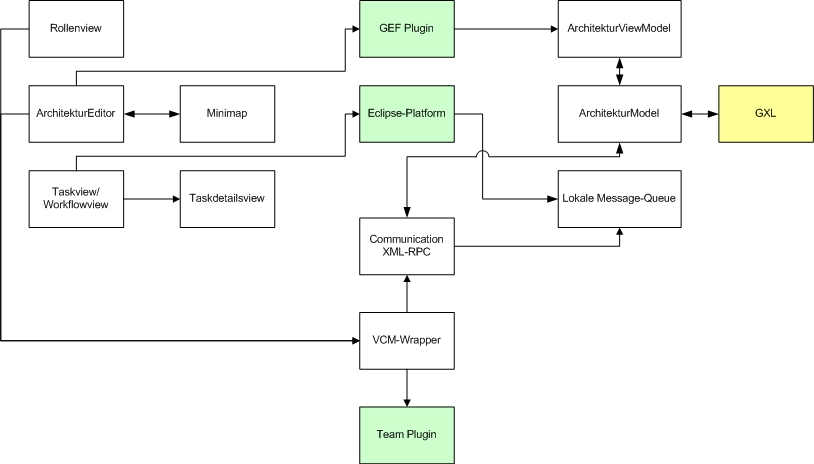
\includegraphics[width=15cm]{client.jpg}

\subsection{MVC-Aufteilung}
Idee des Model-View-Controller Design Patterns ist die Entkopplung der Komponenten
in Gruppen, die ausschlie�lich der Darstellung (View) bzw. Datenhaltung 
(Model) dienen. Die Vermittlung zwischen beiden Gruppen �bernehmen Controller,
so dass die Views und Models keine direkten Abh�ngigkeiten haben.

F�r die Darstellung und Bearbeitung der Architektur ist es notwendig auch 
view-spezifische Informationen f�r den Benutzer zu speichern (z.B. Position 
der Architektur-Elemente), so dass hier ein View-Model zum Einsatz kommt, 
welches das eigentliche Architektur-Model erweitert.\par

Die Aufteilung der Client-Komponenten in MVC-Gruppen sieht wie folgt aus:\par

{\bf View}
\begin{itemize}
    \item Komponente RollenView
    \item Komponente ArchitekturEditor
    \item Komponente Minimap
    \item Komponente Task-/WorkflowView
    \item Komponente TaskDetailView
\end{itemize}\par

{\bf Model}
\begin{itemize}
    \item Komponente ArchitekturModel
    \item Komponente ArchitekturViewModel
    \item Komponente GXL
    \item Komponente MessageQueue
\end{itemize}\par

{\bf Controller}
\begin{itemize}
    \item Delegator-Komponente Server-Kommunikation
    \item Komponente VCM-Wrapper
    \item Komponente GEF (teilweise 3rd-Party)
    \item Komponente Eclipse-Plattform (teilweise 3rd-Party)
    \item Komponente Team-Plugin (teilweise 3rd-Party)
\end{itemize}\par

\section{Viewkomponente RollenView}
Die Rollenview zeigt in einem Baum die Rollen und dazugeh�rigen
Produkte bzw. die zugeh�rige Produktlinie des angemeldeten Benutzers an
(siehe auch 2.1.1. und 2.2.4., Spezifikation I).\par

Die Rollenview operiert �ber die Eclipse-Plattform (ITreeContentProvider) auf der
Komponente ArchitekturModel.

Die Rollenview kann Aktionen in der Komponente VCM-Wrapper ausl�sen sowie
den Architektur-Editor steuern.

\section{Viewkomponente ArchitekturEditor}
Der Architektur-Editor wird mittels der Draw2D und GEF Frameworks realisiert
und stellt die Produktlinienarchitektur gem�� 2.2.2., Spezifikation I
dar.  Er operiert via GEF auf dem ArchitekturViewModel.
Auch die Viewkomponente kann Aktionen des VCM-Wrappers ausf�hren.

\section{Viewkomponente Minimap}
Die Minimap (2.2.3., Spezifikation I) ist direkt mit dem Architektur-Editor 
verkn�pft und stellt eine verkleinerte Fassung der Architektur dar.

\section{Viewkomponente Task-/WorkflowView}
Diese Komponente zeigt die Tasks und Workflows an. Sie operiert �ber die
Controllerkomponente Eclipse-Plattform (IMarker) auf der Komponente MessageQueue.

\section{Viewkomponente TaskDetailView}
Hier werden die Details zu einem Workflow angezeigt. Die Daten werden �ber die
MessageQueue bezogen.

\section{Modelkomponente ArchitekturModel}
Das Architektur-Model enth�lt baumartig aufgebaut alle Informationen �ber die
Produktlinie(n). Das umfasst Varianten, Komponenten, Assets und Benutzer.

\section{Modelkomponente ArchitekturViewModel}
Diese Komponente repr�sentiert auf Modelebene all das, was im Architektur-
Editor angezeigt wird. Das Viewmodel enth�lt zus�tzlich noch Informationen 
�ber die Position der einzelnen Viewelemente auf dem Canvas. Der Aufbau der
ViewModel-Elemente erfolgt dynamisch auf Basis des Architektur-Models und 
durchl�uft Filter, die steuern, welche Elemente tats�chlich angezeigt werden 
sollen. Somit wird eine performantere Darstellung gesichert.

\section{Modelkomponente GXL}
Import und Export der Architekturmodels von und nach GXL.

\section{Modelkomponente MessageQueue}
Diese Komponente ist die lokale Repr�sentation der MessageQueue auf dem Server.
Alle Nachrichten werden �ber die Server-Kommunikations-Komponente bezogen und 
lokal gespeichert. Diese Komponente bedient �ber den Eclipse-Controller die
Task-/Workflow-Viewkomponente.

\section{Controllerkomponente Server-Kommunikation}
Diese Komponente �bernimmt die Kommunikation mit dem Kobold Server. Die 
Kommunikation findet mittels HTTPS (SSL) und XML-RPC statt. Das Querschnitts-
Interface ist unter Kapitel \ref{cha_interface} n�her erl�utert.

\section{Controllerkomponente GEF}
Das Graphical Editing Framework ist ein MVC-basiertes Editing-Framework von 
Eclipse. Der Architektur-Editor setzt darauf auf und kommuniziert �ber dar�ber
mit dem ArchitekturViewModel.

\section{Controllerkomponente Eclipse-Plattform}
Die Eclipse-Plattform bietet viele MVC-unterst�tzende Klassen und Komponenten
mit deren Hilfe die Trennung zwischen Model und View erm�glicht wird.

\section{Controllerkomponente Team-Plugin}
Die Teamplugins sind die Team-Komponenten an die der VCM-Wrapper die Anfragen
weiterdelegiert. In der Eclipse-Plattform ist das CVS-Team-Plugin bereits 
enthalten. Weitere Plugins sind als 3rd-Party-Module verf�gbar.
